% Created 2024-04-03 Wed 10:59
% Intended LaTeX compiler: pdflatex
\documentclass[presentation]{beamer}
\usepackage[utf8]{inputenc}
\usepackage[T1]{fontenc}
\usepackage{graphicx}
\usepackage{longtable}
\usepackage{wrapfig}
\usepackage{rotating}
\usepackage[normalem]{ulem}
\usepackage{amsmath}
\usepackage{amssymb}
\usepackage{capt-of}
\usepackage{hyperref}
\mode<beamer>{\usetheme{Madrid}}
\definecolor{SUred}{rgb}{0.59375, 0, 0.17969} % SU red (primary)
\definecolor{SUblue}{rgb}{0, 0.17578, 0.38281} % SU blue (secondary)
\setbeamercolor{palette primary}{bg=SUred,fg=white}
\setbeamercolor{palette secondary}{bg=SUblue,fg=white}
\setbeamercolor{palette tertiary}{bg=SUblue,fg=white}
\setbeamercolor{palette quaternary}{bg=SUblue,fg=white}
\setbeamercolor{structure}{fg=SUblue} % itemize, enumerate, etc
\setbeamercolor{section in toc}{fg=SUblue} % TOC sections
% Override palette coloring with secondary
\setbeamercolor{subsection in head/foot}{bg=SUblue,fg=white}
\setbeamercolor{date in head/foot}{bg=SUblue,fg=white}
\institute[SU]{Shenandoah University}
\titlegraphic{
\includegraphics[width=0.5\textwidth]{\string~/Documents/suLogo/suLogo.pdf}}
\newcommand{\R}{\mathbb{R}}
\usepackage{tikz}
\usepackage{pgfplots}
\usetheme{default}
\author{Chase Mathison\thanks{cmathiso@su.edu}}
\date{4 April 2024}
\title{Applications of Sequences}
\hypersetup{
 pdfauthor={Chase Mathison},
 pdftitle={Applications of Sequences},
 pdfkeywords={},
 pdfsubject={},
 pdfcreator={Emacs 29.1 (Org mode 9.6.7)}, 
 pdflang={English}}
\begin{document}

\maketitle

\section{Announcements}
\label{sec:orged4d64f}
\begin{frame}[label={sec:orgfb96eae}]{Announcements}
\begin{enumerate}
\item Homework and Project
\item Office hours, 10am - 11am.
\end{enumerate}
\end{frame}

\section{Lecture}
\label{sec:orga0fc616}
\begin{frame}[label={sec:orgb700b43}]{Example}
Let's look at some examples of where sequences come up in real life.

\begin{center}
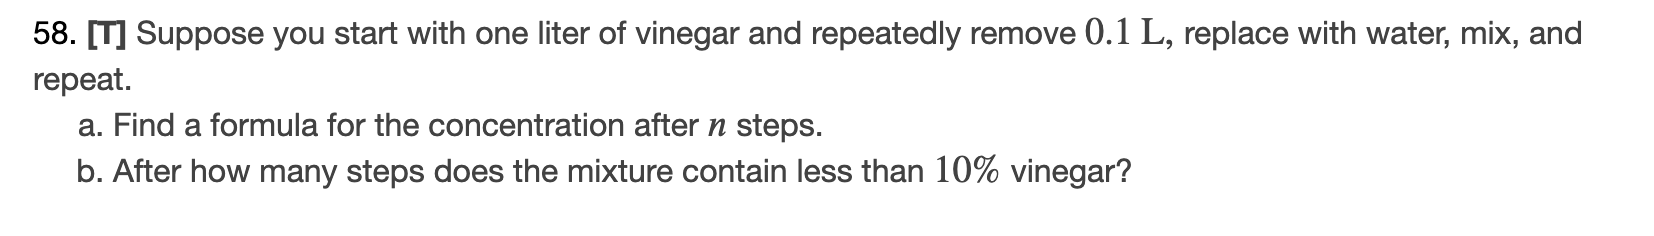
\includegraphics[width=0.7\textwidth]{./q1.png}
\end{center}

\vspace{10in}
\end{frame}

\begin{frame}[label={sec:orgc15c121}]{Example}
\end{frame}

\begin{frame}[label={sec:org0624727}]{Example}
\begin{center}
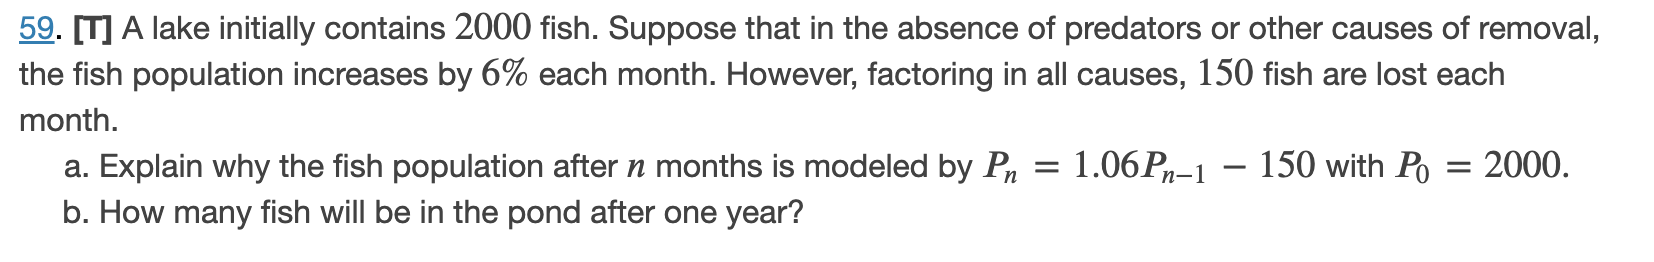
\includegraphics[width=0.7\textwidth]{./q2.png}
\end{center}

\vspace{10in}
\end{frame}

\begin{frame}[label={sec:org4bc8059}]{Example}
\end{frame}

\begin{frame}[label={sec:org7384b0a}]{Example}
\begin{center}
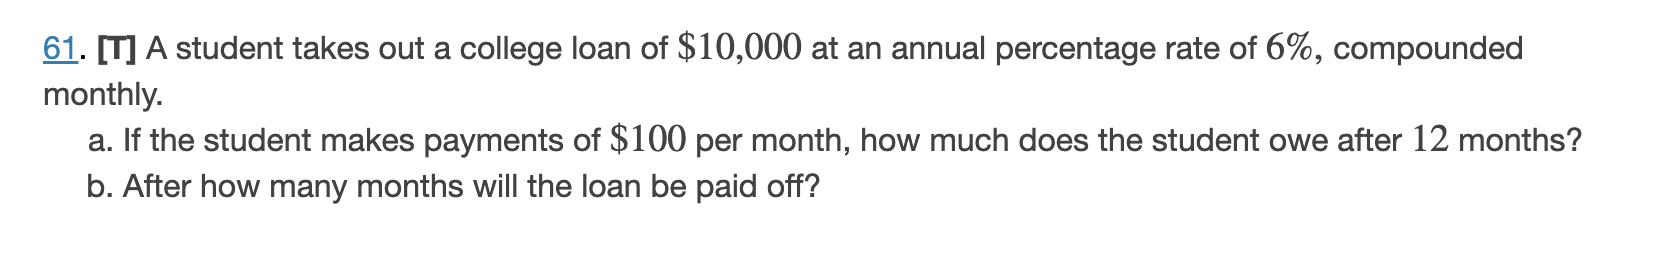
\includegraphics[width=0.7\textwidth]{./q3.png}
\end{center}

\vspace{10in}
\end{frame}

\begin{frame}[label={sec:org9cb8091}]{Example}
\end{frame}

\begin{frame}[label={sec:org2b850b9}]{Example}
Sequences really show up everywhere.  Let's look at one more example of where they show up: The Fibonacci Sequence

\[
F_{n+1} = F_n + F_{n-1},\qquad F_0 = F_1 = 1\]

Let's play around with this sequence for a bit.

\vspace{10in}
\end{frame}

\begin{frame}[label={sec:orgecd89f8}]{Example}
\end{frame}
\end{document}